\section{Tasks}
\subsection{Load and clean dataset}

Due to the fact that the dataset in use was switched since the previous lab, for this tasks the cleaning steps are performed again on the new dataset.

Steps in the cleaning pipeline:
\begin{itemize}
    \item Drop duplicate rows
    \item Separate label column
    \item Coerce features to numeric (non-numeric → NaN)
    \item Impute missing with 0 (common for sparse indicator features)
    \item Drop constant (zero-variance) features
    \item Keep a record of cleaned feature columns
\end{itemize}


\lstinputlisting[style=console,caption={outputs of the cleaning steps},linerange={1-5}]{listings/outputs.txt}

\subsection{Plot label distribution}
\begin{figure}[h]
    \centering
    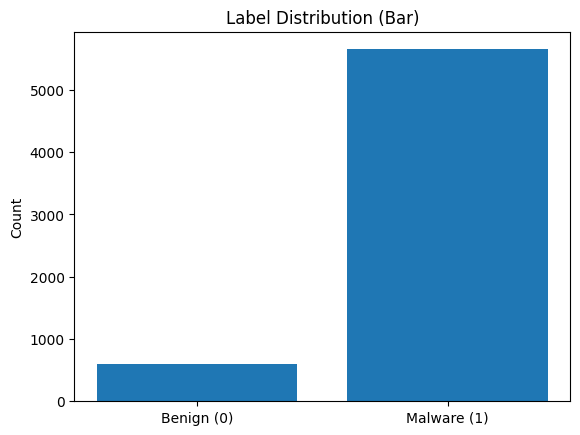
\includegraphics[width=.55\textwidth]{figures/dataset_distribution.png}
    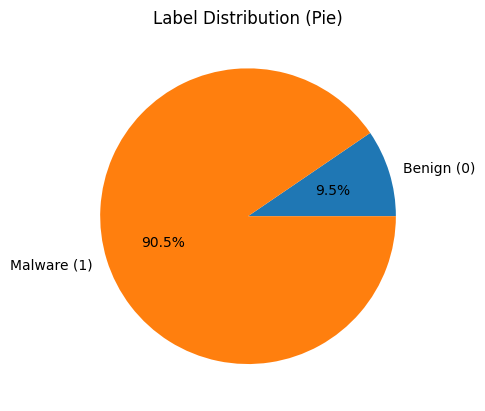
\includegraphics[width=.44\textwidth]{figures/dataset_distribution_pie.png}
    \caption{plots of the dataset label distribution}
    \label{fig:data_dist}
\end{figure}

\subsection{Investigate label imbalance}
\textit{What does your imbalance imply for precision/recall trade-off?}
\vspace{1cm}\\
explanation 123\\

\vspace{1cm}
\textit{How might imbalance affect model training stability?}
\vspace{1cm}\\
explanation 123

\subsection{Data segmentation}
\subsection{Data balancing}